\chapter{Methodology}
\section{Challenges and restrictions}
    \subsection{The .ZARR issue}
        As this thesis was going to be based around the .ZARR format, I soon discovered a problem. 
    \subsection{Bitmap errors} \label{bitmap_error}
        
        
    \subsection{Server at the University of Bergen}
        things
        Restricted creating new data and downloading new, overload of users, hyperparameter search
        
    

\section{My solution}
    \subsection{Pseudo labels} \label{Pseudo label}
        Due to the bitmap errors mentioned in \ref{bitmap_error} I did not have access to the same labels that were used in the original work \ref{unet_paper_acoustic} and had to find an alternate solution. This came to be based on what is called pseudo labels. In meetings with the \gls{imr} we came up with the idea to use the output of the model used in \ref{unet_paper_acoustic} as my labels. This was based on the fact that the models' performance were assessed to be sufficient for my task. I was then able to create as much data with corresponding pseudo labels as I deemed necessary.
        
        This would mean that the labels would consist of predictions produced from the four frequencies used in article \ref{unet_paper_acoustic}, namely; 18kHz,38kHz,120kHz and 200kHz. These values were still in the range 0..1, and so I applied a threshold of 0.8 to convert the values below to 0 and above to 1. Hence, producing a mask for each class \textit{sandeel}, \textit{other} and \textit{background}. Due to the weighted cross-entropy loss used to train the model in section \ref{unet_paper_acoustic} the background class were usually noisy. This was because the weighting caused the model to care less about classifying the background correctly, two samples are illustrated in figure \ref{data sample fig} to illustrate this.
        
        \clearpage
        \begin{figure}[H]
            \centering
            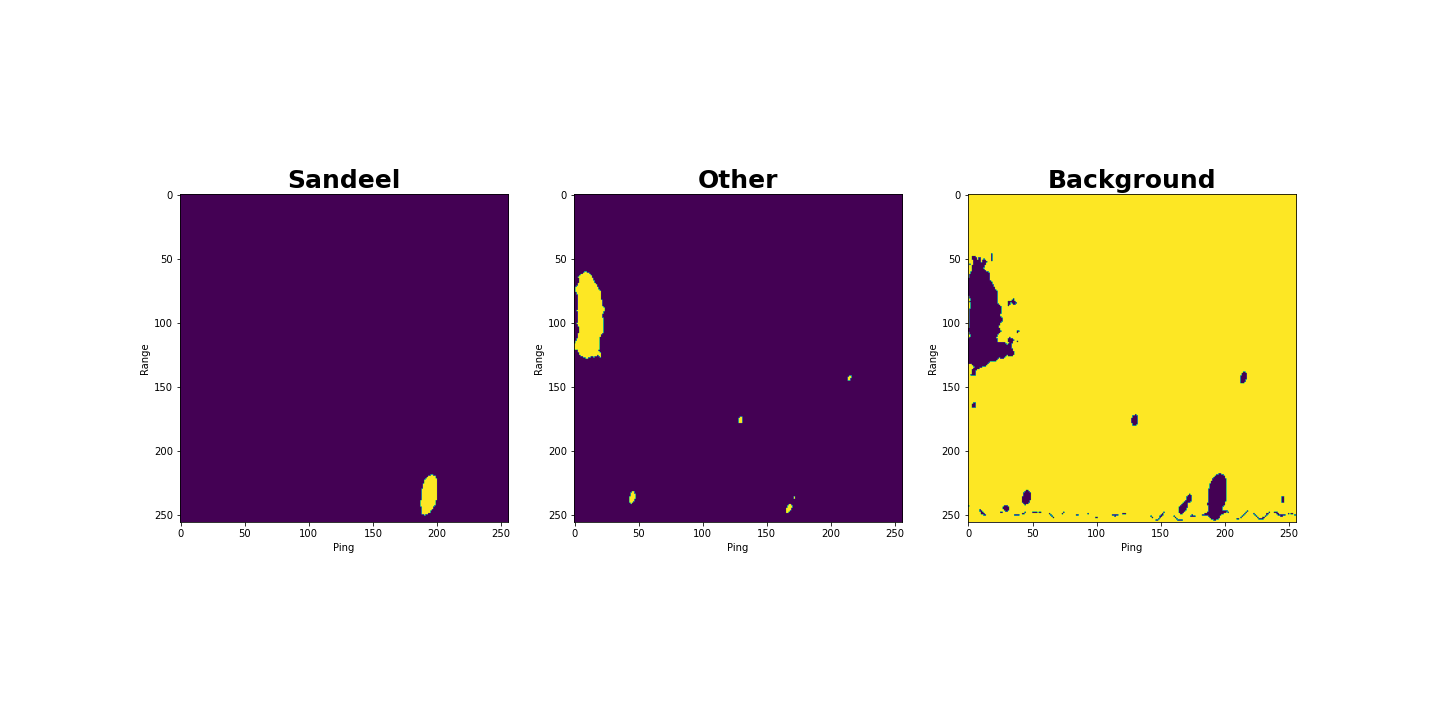
\includegraphics[scale=0.32]{figures/data_sample.png}
          	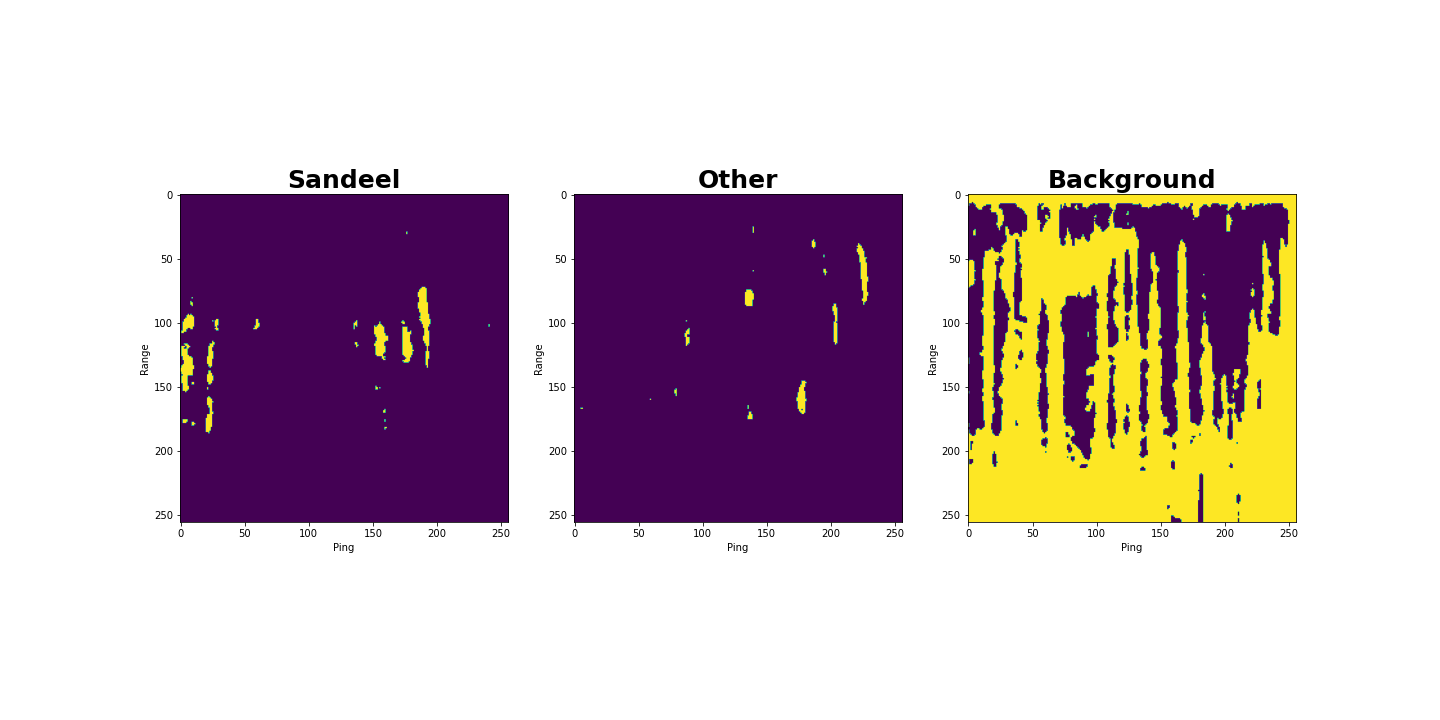
\includegraphics[scale=0.32]{figures/data_sample_noisy.png}
            \caption[Example pseudo label]{Two examples of pseudo labels by row. Purple is values 0 zero and yellow is 1. The upper row illustrates a low noise sample, while the sample in the lower row contains more noise, especially in the background annotations.}
            \label{data sample fig}
        \end{figure}        
        
        
    \subsection{Data generation}
        With the pseudo labels from section \ref{Pseudo label} I possessed all the components I needed to create my own dataset. Here I will go through my implementation of preprocessing the ".RAW" into a dataset able to be quickly loaded into a deep learning algorithm.
        \clearpage
        \begin{figure}[H]
            \centering
            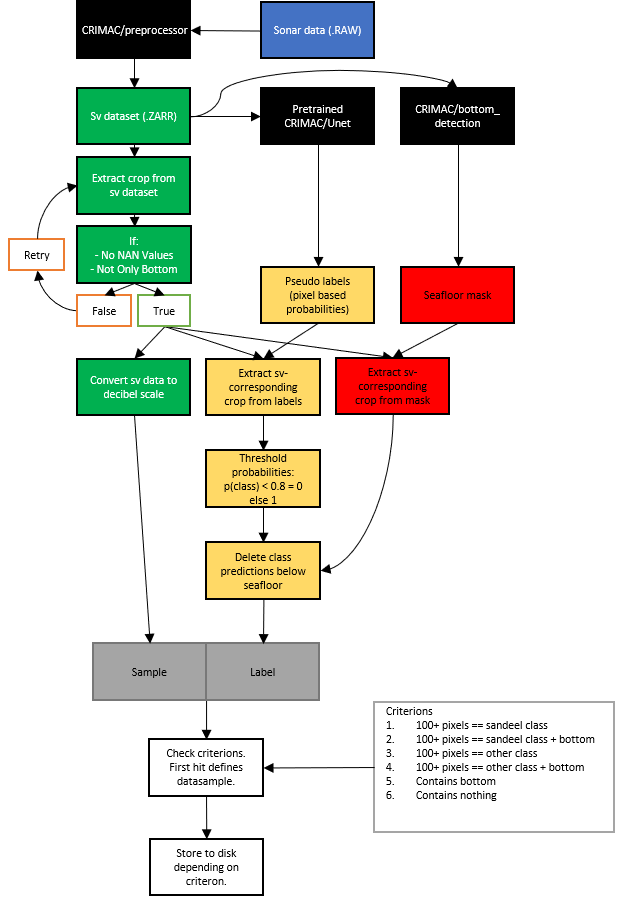
\includegraphics[scale=0.8]{figures/flow_data_gen.png}
            \caption[Data generation process]{An overview of the data generation process. CRIMAC pipeline modules (black), data.raw (blue), SV data.zarr (green), pseudo labels.zarr (yellow), bottom.zarr (red) and the finished file.pytorch (gray)}
          	\medskip 
            \label{data_generation_flowchart_fig}
        \end{figure}
        The entire process is illustrated in figure \ref{data_generation_flowchart_fig} and starts with the utilization of \gls{crimac} preprocessor module as described in \ref{CRIMAC-pipeline}. This takes in the \textit{.RAW} data and outputs the \gls{sv} data in the \textit{.ZARR} format. From the \gls{sv} data, a crop is then extracted and was checked for any missing values or being located entirely below the seafloor. This was repeated until the algorithm found a crop that did not trigger any of the previous two statements.
        
        In figure \ref{data_generation_flowchart_fig} the \gls{sv} data were also sent to both the pretrained U-Net and bottom detection modules from the \gls{crimac} pipeline. The U-Net outputs pseudo labels and the bottom detection outputs a mask of the seafloor. Then, using the vertical and horizontal coordinates from the \gls{sv} data, a corresponding crop from both the seafloor mask and the pseudo labels were extracted. The two new crops were then used together to remove predictions that appeared under the seafloor, thus cleaning the pseudo labels. The steps explained in this paragraph are also visualized in figure \ref{crop_extract_fig}.
        \clearpage
        \begin{figure}[H]
            \centering
            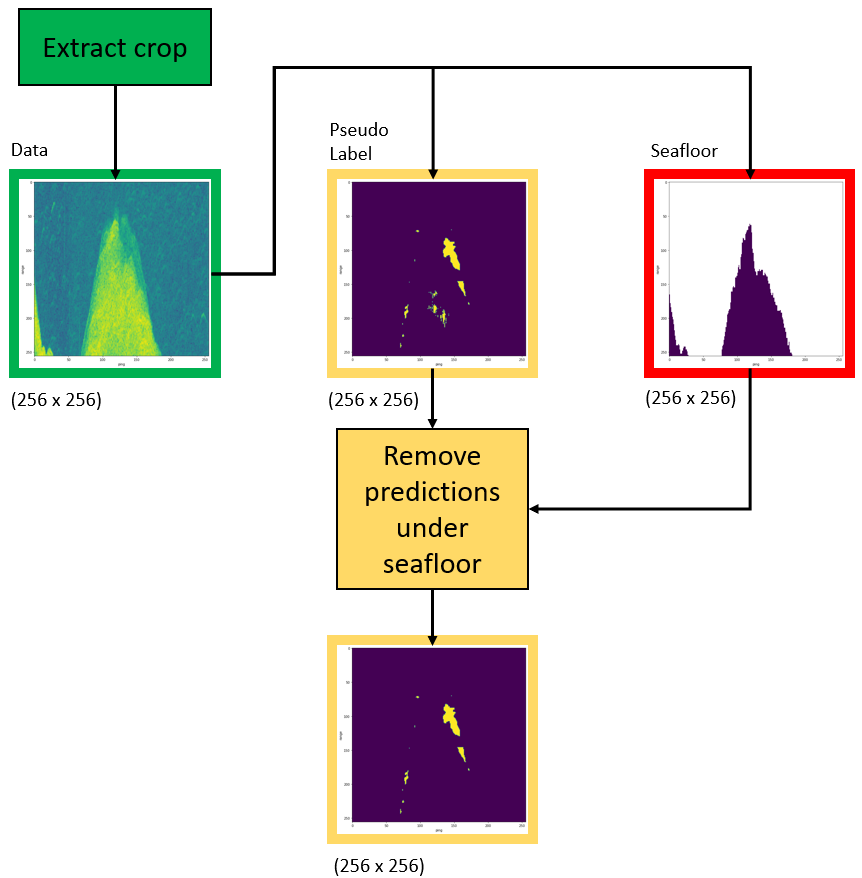
\includegraphics[scale=0.5]{figures/crop_extract_illustration.png}
            \caption[Data, label and bottom crop extraction and interaction]{Example of how the data, pseudo labels and bottom crops would look during data generation. For the pseudo label, purple is values of 0 and yellow value of 1. In the pseudo labels, you can see that some predictions under the seafloor are removed.  Size is shown to make it clear that it is a crop of the same size from the same location.}.
          	\medskip 
            \label{crop_extract_fig}
        \end{figure}
        
        After the crop containing the data and cleaned pseudo labels were generated, I combined them into one file that could be stored to the file system. The file was stored using pytorch (\ref{Pytorch}) based on some criterions that will be explained shortly, creating a data hierarchy as shown in figure \ref{data_hierarchy_fig}:
        
        
        \clearpage
        \begin{figure}[H]
            \centering
            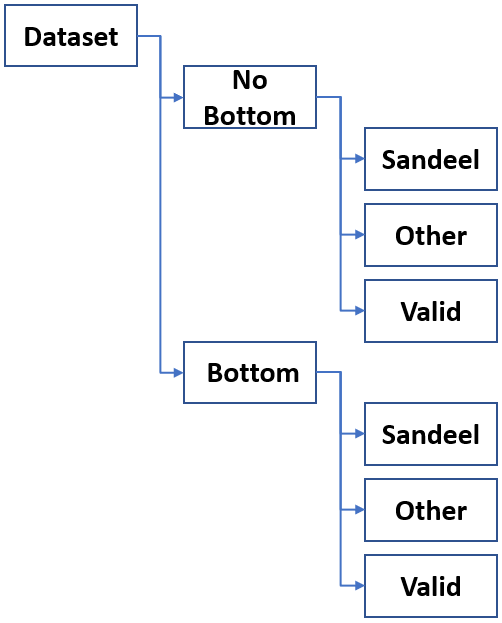
\includegraphics[scale=0.5]{figures/data_hierarki.png}
            \caption[The data-hierarchy]{An overview of the data hierarchy. Two main branches, one with the bottom and one without.}.
          	\medskip 
            \label{data_hierarchy_fig}
        \end{figure}
        
        The criterions were based on those stated in the \ref{unet_paper_acoustic} article and can be seen in figure \ref{data_generation_flowchart_fig}. In the previously mentioned article, they had the real annotations to know if there was \textit{sandeel} or instances of the \textit{other} class in a crop. I had to rely on the pseudo labels for the same task, and as these were noisy, I had to counteract this. Hence, I set a filter where 100 of the pixels in the crop had to belong to a single class to satisfy my criteria. If there were not enough pixels of either class, the crop would be set to be "valid" with or without bottom. To mitigate duplicate samples, the criteria would be checked from the top to the bottom of the criterion list and store the crop to disk depending on the first criterion hit.
        
        The process of generating data from a single year took around 1 to 3 days and close to all capacity on the server. This made me decide to not use all the data, but two years was sufficient for my experiment. In dialogue with the \gls{imr} I chose the year 2018 and 2019 as these were known to have few errors associated with them. The final data distribution can be seen in table \ref{data_distribution_table}.
        
        \clearpage
        \begin{table}[H]
        \caption[Data distribution]{Data distribution for 2019 and 2018.}.
        \begin{tabular}{|llll|l|l|lllll|l|l}
        \cline{1-5} \cline{7-12}
        \multicolumn{4}{|l|}{\textbf{2018 dataset}}                                             & \% of dataset &  & \multicolumn{5}{l|}{\textbf{2019 dataset}}                                             & \% of dataset &  \\ \cline{1-5} \cline{7-12}
        \multicolumn{2}{|l|}{\multirow{3}{*}{No bottom}} & \multicolumn{1}{l|}{Sandeel} & 1410  & 7.3\%         &  & \multicolumn{3}{l|}{\multirow{3}{*}{No bottom}} & \multicolumn{1}{l|}{Sandeel} & 1308  & 4.38\%        &  \\ \cline{3-5} \cline{10-12}
        \multicolumn{2}{|l|}{}                           & \multicolumn{1}{l|}{Other}   & 184   & 0.95\%        &  & \multicolumn{3}{l|}{}                           & \multicolumn{1}{l|}{Other}   & 1074  & 3.60\%         &  \\ \cline{3-5} \cline{10-12}
        \multicolumn{2}{|l|}{}                           & \multicolumn{1}{l|}{Valid}   & 6519  & 33.75\%       &  & \multicolumn{3}{l|}{}                           & \multicolumn{1}{l|}{Valid}   & 10291 & 34.45\%       &  \\ \cline{1-5} \cline{7-12}
        \multicolumn{2}{|l|}{\multirow{3}{*}{Bottom}}    & \multicolumn{1}{l|}{Sandeel} & 1297  & 6.71\%        &  & \multicolumn{3}{l|}{\multirow{3}{*}{Bottom}}    & \multicolumn{1}{l|}{Sandeel} & 1652  & 5.53\%        &  \\ \cline{3-5} \cline{10-12}
        \multicolumn{2}{|l|}{}                           & \multicolumn{1}{l|}{Other}   & 840   & 4.35\%        &  & \multicolumn{3}{l|}{}                           & \multicolumn{1}{l|}{Other}   & 2815  & 9.42\%        &  \\ \cline{3-5} \cline{10-12}
        \multicolumn{2}{|l|}{}                           & \multicolumn{1}{l|}{Valid}   & 9067  & 46.94\%       &  & \multicolumn{3}{l|}{}                           & \multicolumn{1}{l|}{Valid}   & 12733 & 42.62\%       &  \\ \cline{1-5} \cline{7-12}
        \multicolumn{3}{|l|}{\textbf{Total}}                                            & 19317 & 100\%         &  & \multicolumn{4}{l|}{\textbf{Total}}                                            & 29873 & 100\%         &  \\ \cline{1-5} \cline{7-12}
        \end{tabular}
        \label{data_distribution_table}
        \end{table}
        
        From the table \ref{data_distribution_table} I observed that as in article \ref{unet_paper_acoustic} most of the data will contain no fish, here represented as "valid".
        
\section{Experiments}
    The experiments revolved around manipulating the amount of frequencies given as input to the model. In this section, I will describe how my experiments were performed and my thought process around evaluation performance. 
    
    \subsection{Experiment settings} \label{Experiment settings}
        All models are based on the one created in article \ref{unet_paper_acoustic}. This means the architecture, hyperparameters and the way the data is loaded into the model. A summary can be seen in table \ref{experiment_settings_table}.


\clearpage
\begin{longtable}{lcl}
\hline
\multicolumn{1}{|l|}{\textbf{Sample class}} & \multicolumn{1}{l|}{\textbf{Probability}} & \multicolumn{1}{l|}{\textbf{Details}}                                                         \\ \hline
\endfirsthead
%
\endhead
%
Sandeel                                     & 5/26                                      & Random crop containing the sandeel class                                                      \\ \hline
Other                                       & 5/26                                      & Random crop containing the other class                                                        \\ \hline
Valid                                       & 1/26                                      & Random crop containing no fish                                                                \\ \hline
Sandeel + bottom                          & 5/26                                      & \begin{tabular}[c]{@{}l@{}}Random crop containing the sandeel class\\ + seafloor\end{tabular} \\ \hline
Other + bottom                             & 5/26                                      & \begin{tabular}[c]{@{}l@{}}Random crop containing the other class\\ + seafloor\end{tabular}   \\ \hline
Valid + bottom                        & 5/26                                      & \begin{tabular}[c]{@{}l@{}}Random crop containing no fish\\ + seafloor\end{tabular}           \\ \hline
\end{longtable}


\clearpage
\begin{longtable}{lll}
\hline
\multicolumn{1}{|l|}{\textbf{Hyperparameters}} & \multicolumn{1}{l|}{\textbf{Value/ Category}} & \multicolumn{1}{l|}{\textbf{Details}}                                                 \\ \hline
\endfirsthead
%
\endhead
%
\textit{Loss function:}                         & Weighted Cross-entropy                        & \begin{tabular}[c]{@{}l@{}}Background = 1, \\ Other = 25,\\ Sandeel = 30\end{tabular} \\ \hline
\textit{Optimizer:}                             & Stochastic gradient descent                   &                                                                                       \\ \hline
\textit{Learning rate:}                         & 0.01                                          & \begin{tabular}[c]{@{}l@{}}Halved every \\ 1000th batch\end{tabular}                  \\ \hline
\textit{Momentum:}                              & 0.95                                          &                                                                                       \\ \hline
\textit{Batch size:}                            & 16                                            &                                                                                       \\ \hline
\textit{Crop size:}                             & 256x256                                       & \begin{tabular}[c]{@{}l@{}}Include all \\ available channels\end{tabular}             \\ \hline
\end{longtable}


\clearpage
\begin{longtable}{lll}
\hline
\multicolumn{2}{|l|}{\textbf{Data augmentation}} & \multicolumn{1}{l|}{\textbf{Details}} \\ \hline
\endfirsthead
%
\endhead
%
\textit{Add noise to 5\% of pixels}      &       & 50\% of happening upon loading sample \\ \hline
\textit{Flip along vertical axis}        &       & 50\% of happening upon loading sample \\ \hline
\textit{Convert to decibel scale}        &       & Min -75db, max 0db                    \\ \hline
\end{longtable}

        
        For all experiments, the model architecture was based on the one described in section \ref{unet_paper_acoustic}. The only change to the model was the number of channels in the input layer called "input image" with a value of 4 in figure \ref{unet_fig}. This would range from 1 to 6 to accommodate the tests.
        
        To evaluate the performance of the models, I utilized the F1 score mentioned in section \ref{f1_score}. I also included the precision and recall, as these are interesting values to discuss and gives greater insight.
        
    %\subsection{Experiment: Training on pseudo labels}
    %  This was a preliminary test to establish that training a model on pseudo labels was possible and would achieve acceptable performance. All frequencies would be included, and this would then produce a baseline performance for the later experiments. 
    
    \subsection{Experiment: Exhaustive frequency search}
        To find the most impactful frequencies and try to discover hidden synergies between them, a comprehensive test had to be enacted. This experiment would see all combinations of all frequencies being tested. A total of 5 separate tests would be run to reduce variance in the results. Each would have different random state seeds set to enable different model initialization, but mainly the data would not be identical due to the new sequence loaded and augmentations applied. The random state also accommodates reproducibility. With 6 frequencies in total, the amount of possible combinations for each of the 5 testes would be 63, as the order did not matter.
        
        I observed that the year 2019 in table \ref{data_distribution_table} had the most data, and this was to be the one used during training. 70\% was to be training data, and 30\% as validation data. The 2018 dataset was set as the test data. The total amount of data was 5,000 batches. With a batch size of 16 this corresponds to 80,000 samples ($5,000 * 16$). This was the same amount as used in the \gls{crimac} U-Net model (section \ref{unet_paper_acoustic})
        
        Logging of metrics would occur at different stages during the training process;
            \begin{itemize}
                \item Every 100 minibatch: Record training loss.
                \item Every 500 minibatch: Run model on 100 batches from the validation data, plot one sample output, its label and record validation loss. Also, calculate F1-score on both training and validation data for every class, and add the historical F1-scores for the sandeel class to the plot. 
            \end{itemize}
    
        As the logging and random state was equal for all combinations internal in a test, this would create good comparison illustrations. The metrics loss and F1-score would give an indication towards convergence, over-/under-fitting problems and performance.
        
        After the training of the current combination, the network would be evaluated on 500 batches from the test data, but without any noise added through augmentation. Vertical flipping would still occur. Finally, the F1-score, precision and recall would be calculated for each class and logged in a \textit{.csv} file. Then the next combination would start the entire process afresh with training.
        
        
        
    \subsection{Experiment: Greedy-search frequencies - Decreasing amount}
        This experiment will look into the performance of a model that both trains and predicts on data containing sequentially fewer frequencies. 
        
        
    \subsection{Experiment: Greedy-search frequencies - Increasing amount}
    
        

